\documentclass{sig-alternate}
\usepackage{epsfig}

%%  \toappear{
%%  %\raisebox{2pt}[2pt]{\underline{~~~~~~~~~~~~~~~~~~~~~~~~~~~~~~~~~~~~~~~~~~~~~~~~~~}} \\
%%  %$^*$ More information on the StreamIt project is available from
%%  %\texttt{http://compiler.lcs.mit.edu/streamit} \\
%%    \rule{0cm}{0cm}\\\hrule\rule{0cm}{0cm} ~ \\ \vspace{-6pt} ~ \\
%%  \parbox[b]{20pc}{\baselineskip 9pt
%%  Permission to make digital or hard copies of all or part of this work
%%  for personal or classroom use is granted without fee provided that
%%  copies are not made or distributed for profit or commercial advantage
%%  and that copies bear this notice and the full citation on the first
%%  page.  To copy otherwise, to republish, to post on servers or to
%%  redistribute to lists, requires prior specific permission and/or a
%%  fee.} \par
%%  {\it PLDI'03}, June 9--11, 2003, San Diego, California, USA. \par
%%  Copyright 2003 ACM 1-58113-662-5/03/0006 ...\$5.00 \\ ~ \\ ~ \\
%% }

\title{Teleport Messaging for Distributed Stream Programs}
%\title{Stream Dependence Analysis and its \\ Application to Precise Event Handling}

\numberofauthors{1}
\author{
  \alignauthor{\mbox{\hspace{-20pt}William Thies, Michal Karczmarek, Janis Sermulins, Rodric Rabbah, and Saman Amarasinghe}}\\
%  \alignauthor{William Thies, Michal Karczmarek, Janis Sermulins, \\ Rodric Rabbah, and Saman Amarasinghe}\\
  \email{\raisebox{0.5pt}{{\large\{}}thies, karczma, janiss, rabbah, saman\raisebox{0.5pt}{{\large\}}}@csail.mit.edu}\\[0.4Ex]
  \affaddr{Computer Science and Artificial Intelligence Laboratory}\\[0.3Ex]
  \affaddr{Massachusetts Institute of Technology}
}

%% \numberofauthors{5}
%% \author{
%% %
%% % The command \alignauthor (no curly braces needed) should
%% % precede each author name, affiliation/snail-mail address and
%% % e-mail address. Additionally, tag each line of
%% % affiliation/address with \affaddr, and tag the
%% %% e-mail address with \email.
%% \alignauthor Ben Trovato\titlenote{Dr.~Trovato insisted his name
%% be first.}\\
%%        \affaddr{Institute for Clarity in Documentation}\\
%%        \affaddr{1932 Wallamaloo Lane}\\
%%        \affaddr{Wallamaloo, New Zealand}\\
%%        \email{trovato@corporation.com}
%% \alignauthor G.K.M. Tobin\titlenote{The secretary disavows
%% any knowledge of this author's actions.}\\
%%        \affaddr{Institute for Clarity in Documentation}\\
%%        \affaddr{P.O. Box 1212}\\
%%        \affaddr{Dublin, Ohio 43017-6221}\\
%%        \email{webmaster@marysville-ohio.com}
%% \alignauthor Lars Th{\Large{\sf{\o}}}rv{$\ddot{\mbox{a}}$}ld\titlenote{This author is the
%% one who did all the really hard work.}\\
%%        \affaddr{The Th{\large{\sf{\o}}}rv{$\ddot{\mbox{a}}$}ld Group}\\
%%        \affaddr{1 Th{\large{\sf{\o}}}rv{$\ddot{\mbox{a}}$}ld Circle}\\
%%        \affaddr{Hekla, Iceland}\\
%%        \email{larst@affiliation.org}
%% }
%% \additionalauthors{Additional authors: John Smith (The Th{\o}rv\"{a}ld Group,
%% email: {\texttt{jsmith@affiliation.org}}) and Julius P.~Kumquat
%% (The Kumquat Consortium, email: {\texttt{jpkumquat@consortium.net}}).}

\begin{document}

\conferenceinfo{PPoPP'05,} {June 15--17, 2005, Chicago, Illinois, USA.}
\CopyrightYear{2005}
\crdata{1-59593-080-9/05/0006} 

%%%%%%%%%%%%%%%%%%%%%%%%%%%%%%%%%%%%%%%%%%%%%%%%%%%%%%%%%%%%%%%%%%%%%%%%%%

\newtheorem{definition}{Definition}
\newtheorem{theorem}{Theorem}
\newtheorem{algorithm}{Algorithm}

\maketitle

\newcommand{\figsdep}[0]{\mt{SDEP}}
\newcommand{\figsdepf}[2]{\mt{SDEP}_{#1 \small{\leftarrow} #2}}
\newcommand{\sdep}[0]{\textsc{sdep}}
\newcommand{\sdepf}[2]{\sdep_{#1 \small{\leftarrow} #2}}
\newcommand{\floor}[2]{\left\lfloor\frac{#1}{#2}\right\rfloor}
\newcommand{\ceil}[2]{\left\lceil\frac{#1}{#2}\right\rceil}

\newcommand{\mt}[1]{\mbox{\it #1}}
\newcommand{\todo}[1]{\framebox{\bf #1}}
\newcommand{\naive}[0]{na\"{\i}ve}
\newcommand{\Naive}[0]{Na\"{\i}ve}
\newcommand{\makeline}[0]{\rule{0cm}{0cm}\\\hrule\rule{0cm}{0cm}}

\begin{abstract}
In this paper, we develop a new language construct to address one of
the pitfalls of parallel programming: precise handling of events
across parallel components.  The construct, termed {\it teleport
messaging}, uses data dependences between components to provide a
common notion of time in a parallel system.  Our work is done in the
context of the Synchronous Dataflow (SDF) model, in which computation
is expressed as a graph of independent components (or {\it actors})
that communicate in regular patterns over data channels.  We leverage
the static properties of SDF to compute a stream dependence function,
$\sdep$, that compactly describes the ordering constraints between
actor executions.

Teleport messaging utilizes $\sdep$ to provide powerful and precise
event handling.  For example, an actor $A$ can specify that an event
should be processed by a downstream actor $B$ as soon as $B$ sees the
``effects'' of the current execution of $A$.  We argue that teleport
messaging improves readability and robustness over existing practices.
We have implemented messaging as part of the StreamIt compiler, with a
backend for a cluster of workstations.  As teleport messaging exposes
optimization opportunities to the compiler, it also results in a 49\%
performance improvement for a software radio benchmark.

\end{abstract}

\category{D.3.3}{Programming Languages}{Language Constructs and Features}
\category{D.3.2}{Programming Languages}{Language Classifications}[Concurrent, distributed, and parallel languages; Data-flow languages]
%\category{D.1.3}{Programming Techniques}{Concurrent Programming}
%\category{D.2.2}{Software Engineering}{Software Architectures}
%\category{D.3.4}{Programming Languages}{Processors}
%\category{D.2.2}{Software Engineering}{Design Tools and Techniques}

\begin{terms}
Languages, Design, Performance
\end{terms}

\begin{keywords}
StreamIt, Synchronous Dataflow, Event Handling, Dependence Analysis,
Digital Signal Processing, Embedded
\end{keywords}
\section{Introduction}

Algorithms that operate on streams of data are becoming increasingly
pervasive across a broad range of applications, and there is evidence
that streaming media applications already consume a substantial
fraction of the computation cycles on consumer
machines~\cite{conte97,dief97,kirkpatrick97,Rix98}.  Examples of
streaming workloads can be found in embedded systems (e.g., sensor
nets and mobile phones), as well as in desktop machines (e.g.,
networking and multimedia) and high-performance servers (e.g., HDTV
editing consoles and hyper-spectral imaging).

As high performance remains a critical factor for many streaming
applications, programmers are often forced to sacrifice readability,
robustness, and maintainability of their code for the sake of
optimization.  One notoriously difficult aspect of stream programming,
from both a performance and programmability standpoint, is reconciling
regular streaming dataflow with irregular control messages.  While the
high-bandwidth flow of data is very predictable, realistic
applications also include unpredictable, low-bandwidth control
messages for adjusting system parameters (e.g., filtering
coefficients, frame size, compression ratio, network protocol, etc.).
Control messages often have strict timing constraints that are
difficult to reason about on parallel systems.

For example, consider a frequency hopping radio (FHR), which mirrors
how CDMA-based cell phone technology works.  In FHR, a transmitter and
a receiver switch between a set of known radio frequencies, and they
do so in synchrony with respect to a stream boundary. That is, a
receiver must switch its frequency at an exact point in the stream (as
indicated by the transmitter) in order to follow the incoming signal.
Such a receiver is challenging to implement in a distributed
environment because different processors might be responsible for the
radio frontend and the frequency hop detection.  When a hop is
detected, the detector must send a message to the frontend that is
timed precisely with respect to the data stream, even though the two
components are running on different processors with independent
clocks.

Other instances of control messaging have a similar flavor.  A
component in a communications frontend might detect an invalid
checksum for a packet, and send a precisely-timed message downstream
to invalidate the effects of what has been processed.  Or, a
downstream component might detect a high signal-to-noise ratio and
send a message to the frontend to increase the amplification.  In an
adaptive beamformer, a set of filtering coefficients is periodically
updated to focus the amplification in the direction of a moving
target.  Additional examples include: periodic channel
characterization; initiating a handoff (e.g., to a new network
protocol); marking the end of a large data segment; and responding to
user inputs, environmental stimuli, or runtime exceptions.

There are two common implementation strategies for control messages
using today's languages and compilers.  First, the message can be
embedded in the high-bandwidth data stream, perhaps as an extra field
in a data structure.  Application components check for the presence of
messages on every iteration, processing any that are found.  This
scheme offers precise timing across distributed components, as the
control message has a well-defined position with respect to the data
stream.  However, the timing is inflexible: it is impossible for the
sender to synchronize the message delivery with a data item that has
already been sent, or to send messages upstream, against the flow of
data.  In addition, this approach adds complexity and runtime overhead
to the steady-state data processing, and it requires a direct
high-bandwidth connection between sender and receiver.

A second implementation strategy is to perform control messaging
``out-of-band'', via a new low-bandwidth connection or a remote
procedure call.  While this avoids the complexity of embedding
messages in a high-bandwidth data stream, it falls short in terms of
timing guarantees.  In a distributed environment, each processor has
its own clock and is making independent progress on its part of the
application.  The only common notion of time between processors is the
data stream itself.  Though extra synchronization can be imposed to
keep processors in check, such synchronization is costly and can
needlessly suppress parallelism.  Also, the presence of dynamic
messaging can invalidate other optimizations which rely on static
communication patterns.

This paper presents a new language construct and supporting compiler
analysis that allows the programmer to declaratively specify control
messages.  Termed ``teleport messaging'', this feature offers the
simplicity of a method call while maintaining the precision of
embedding messages in the data stream.  The idea is to treat control
messages as an asynchronous method call with no return value.  When
the sender calls the method, it has the semantics of embedding a
placeholder in the sender's output stream.  The method is invoked in
the receiver when the receiver would have processed the placeholder.
We generalize this concept to allow messages both upstream and
downstream, and with variable latency.  By exposing the true
communication pattern to the compiler, the message can be delivered
using whatever mechanism is appropriate for a given architecture.  The
declarative mechanism also enables the compiler to parallelize and
reorder application components so long as it delivers messages on
time.

Our formulation of teleport messaging relies on a restricted model of
computation known as Synchronous Dataflow, or SDF~\cite{LM87-i}.  As
described in Section~\ref{sec:sdf}, SDF expresses computation as a
graph of communicating components, or {\it actors}.  A critical
property of SDF is that the input and output rate of each actor is
known at compile time.  Using this property, we can compute the
dependences between actors and automatically calculate when a message
should be delivered.  We develop a stream dependence function,
$\sdep$, that provides an exact, complete, and compact representation
of this dependence information; we use $\sdep$ to specify the
semantics of teleport messaging.

Teleport messaging is implemented as part of the StreamIt compiler
infrastructure~\cite{streamitcc}.  The implementation computes $\sdep$
information and automatically targets a cluster of workstations.
Based on a case study of a frequency hopping radio, we demonstrate a
49\% performance improvement due to communication benefits of teleport
messaging.  As described in Section~\ref{sec:constraints}, our
implementation limits certain sender-receiver pairs to be in distinct
portions of the stream graph; if overlapping messages are sent with
conflicting latencies, it may be impossible to schedule the delivery.
This constrained scheduling problem is an interesting topic for future
work.

This paper is organized as follows.  In the rest of this
section, we describe our model of computation and give a concrete
example of teleport messaging.  Section~\ref{sec:sdep} defines the
stream dependence function, and Section~\ref{sec:calc-sdep} shows how
to calculate it efficiently.  Section~\ref{sec:teleport} gives the
semantics for teleport messaging, and Section~\ref{sec:casestudy}
describes our case study and implementation results.  
%Other
%applications for $\sdep$ appear in Section~\ref{sec:others-apps},
Related work appears in Section~\ref{sec:related-work}, while
conclusions and future work appear in Section~\ref{sec:conclusion}.

%% In  this  paper, we focus on the 
%% computation paradigm embodied by Synchronous  Dataflow~\cite{LM87-i},
%% a popular  model  that  is well suited for  streaming codes.  
%% In this model, computation is represented  as a structured graph consisting
%% of {\it actors} connected by communication channels.

% which describes the
% ordering constraints of actor firings in an SDF graph.  This
% dependence information is similar to a program slice, which has a rich
% body of work surrounding it~\cite{hrb88pdg,pugh97slice,tip95slice}.
% Like program slicing, $\sdep$ can also facilitate debugging and
% program analysis.  However, unlike program slicing, one can leverage
% the static properties of SDF 
% Our work  is presented  in the context  of Synchronous  Dataflow (SDF)
% which  is a popular  model of  computation~\cite{LM87-i} that  is well
% suited for  streaming codes. In  SDF, computation is represented  as a
% graph consisting of {\it  actors} connected by communication channels;
% the actors consume  and produce a constant number  of items from their
% input and output  channels every time they execute.   SDF is appealing
% because it is ameable to static scheduling and optimization.
% However, the challenge
% comes when there is a dynamic, unpredictable event in the stream; for
% instance, an actor detects a low signal-to-noise ratio and sends a
% signal to the frontend to increase the amplification.  How should the
% control message be delivered?  The problem is further complicated when
% there is a constraint on the timing of the message.  With the abundant
% parallelism in stream programs, how can concurrent actors have a
% common frame of reference with respect to time?
%% This paper makes two contributions towards this goal.  First, we
%% formulate a stream dependence function, $\sdep$, which describes the
%% ordering constraints of node executions in a concurrent stream graph.
%% This dependence information is similar to a program
%% slice~\cite{tip95slice,hrb88pdg} in procedural programs and carries
%% with it many of the applications of slicing, including debugging and
%% program analysis.  However, unlike slicing, we restrict our input
%% domain to a Synchronous Dataflow (SDF) ~\cite{LM87-i} graph, which is
%% a natural representation for many signal processing applications.  We
%% leverage the static properties of SDF to compute $\sdep$ exactly at
%% compile time and to store the dependence information compactly.

%% The second contribution of this paper is a novel language construct
%% that uses $\sdep$ to provide simple and precise event handling in
%% stream programs.  In addition to the high-bandwidth data flow of
%% streaming applications, there are also low-bandwidth control messages
%% that adjust parameters in the stream graph; for example, toggling the
%% gain to suite the signal-to-noise ratio, or steering a microphone
%% array to follow a moving target.  Control messages are dynamic and
%% irregular, which makes them hard to integrate with a Synchronous
%% Dataflow model.  Most of all, they often have a constraint on the
%% timing of their delivery, which further complicates the programming
%% model because concurrent actors have no common frame of reference with
%% respect to time.
				   
%% We define a messaging construct that utilizes data dependences 

\subsection{Model of Computation}
\label{sec:sdf}

%% Our model of computation is Synchronous Dataflow~\cite{LM87-ii}, which
%% is well suited for signal processing applications.  Computation is
%% represented as a graph of {\it actors} connected by FIFO communication
%% channels.  We also support a generalization of SDF known as
%% Cyclo-Static Dataflow (CSDF), in which each actor follows a set of
%% execution steps, or phases~\cite{BELP96}.  Like actors in SDF, each
%% phase in CSDF consumes a constant number of items from each input
%% channel and produces a constant number of items onto each output
%% channel.  The number and ordering of phases is known at compile time,
%% and their execution is cyclic (that is, after executing the last
%% phase, the first phase is executed again).  Synchronous Dataflow is
%% appealing because every actor has fixed input and output rates, making
%% the stream graphs amenable to static scheduling and
%% optimization~\cite{LM87-i}.

Our model of computation is Cyclo-Static Dataflow (CSDF), a
generalization~\cite{BELP96} of Synchronous Dataflow, or
SDF~\cite{LM87-i}.  SDF and its variants are well suited for signal
processing applications. Computation is represented as a graph of {\it
actors} connected by FIFO communication channels.  In CSDF, each actor
follows a set of execution steps, or phases.  Each phase consumes a
fixed number of items from each input channel and produces a fixed
number of items onto each output channel.  The number and ordering of
phases is known at compile time, and their execution is cyclic (that
is, after executing the last phase, the first phase is executed
again).  If each actor has only one phase, then CSDF is equivalent to
SDF.  These models are appealing because the fixed input and output
rates make the stream graph amenable to static scheduling and
optimization~\cite{LM87-i}.

In this paper, we use the StreamIt programming
language~\cite{streamitcc} to describe the connectivity of the
dataflow graph as well as the internal functions of each actor.  Our
technique is general and should apply equally well to other languages
and systems based on Synchronous or Cyclo-Static Dataflow.  In
StreamIt, each actor (called a {\it filter} in the language) has one
input channel and one output channel.  An execution step consists of a
call to the ``work function'', which contains general-purpose code.
During each invocation, an actor consumes ({\it pops}) a fixed number
of items from the input channel and produces ({\it pushes}) a fixed
number of items on the output channel.  It can also {\it peek} at
input items without consuming them from the channel.

Actors are assembled into single-input, single-output stream graphs
(or {\it streams}) using three hierarchical primitives.  A {\it
pipeline} arranges a set of streams in sequence, with the output of
one stream connected to the input of the next.  A {\it splitjoin}
arranges streams in parallel; incoming data can either be duplicated
to all streams, or distributed using a round-robin splitter.
Likewise, outputs of the parallel streams are serialized using a
round-robin joiner.  Round-robin splitters (resp. joiners) execute in
multiple phases: the $i$th phase pushes (resp. pops) a known number of
items $k_i$ to (resp. from) the $i$th stream in the splitjoin.
Finally, a {\it feedbackloop} can be used to introduce cycles in the
graph.

\subsection{Illustrating Example}

Figure~\ref{fig:fir-orig-code} illustrates a StreamIt version of an
FIR (Finite Impulse Response) filter.  A common component of digital
%
\begin{figure*}[t]
\begin{minipage}[b]{150pt}
\psfig{figure=fir-orig.eps,scale=0.45}
\end{minipage}
\begin{minipage}[b]{300pt}
\psfig{figure=fir-struct.eps,scale=0.45}~~~~~
\psfig{figure=fir-messaging.eps,scale=0.45}
\end{minipage}

\begin{minipage}{150pt}
  \caption{FIR code.
    \protect\label{fig:fir-orig-code}}
~\\
\end{minipage}~~
\begin{minipage}{153pt}
  \caption{FIR code with manual event handling.  Modified lines are marked with an asterisk.
    \protect\label{fig:fir-manual-code}}
\end{minipage}~~~~~
\begin{minipage}{145pt}
  \caption{FIR code with teleport messaging.  Modified lines are marked with an asterisk.
    \protect\label{fig:fir-message-code}}
\end{minipage} \vspace{2\baselineskip}

\begin{minipage}[t]{0.74in}
\begin{center}
\psfig{figure=fir1.eps,width=0.629in}
\end{center}
\end{minipage}
\hspace{0.15in}
\begin{minipage}[t]{3.04in}
\begin{center}
\psfig{figure=fir2.eps,width=3.04in}
\end{center}
\end{minipage}
\hspace{0.11in}
\begin{minipage}[t]{2.95in}
\begin{center}
\psfig{figure=fir3.eps,width=2.915in}
\end{center}
\end{minipage}

\begin{minipage}[t]{0.74in}
\mbox{~}
\caption{FIR stream graph.\protect\label{fig:fir-orig-diagram}}
\end{minipage}
\hspace{0.2in}
\begin{minipage}[t]{2.9in}
\mbox{~}\hspace{0.045in}{\bf (a)}
~\hspace{0.368in}{\bf (b)}
~\hspace{0.345in}{\bf (c)}
~\hspace{0.345in}{\bf (d)}
~\hspace{0.345in}{\bf (e)}
\caption{Execution snapshots illustrating manual embedding of control
messages in FIR.  Channels are annotated with data items present on
one possible execution; items are numbered in order of production.
{\bf (a)} Source initiates change of weights, {\bf (b)} weights are
attached to data item \#5 and embedded in stream, {\bf (c)-(e)},
actors check each input item, adjusting their own weight when they
find a tagged item.\protect\label{fig:fir-manual-diagram}}
\end{minipage}
\hspace{0.25in}
\begin{minipage}[t]{2.85in}
\mbox{~}\hspace{0.065in}{\bf (a)}
~\hspace{0.325in}{\bf (b)}
~\hspace{0.325in}{\bf (c)}
~\hspace{0.325in}{\bf (d)}
~\hspace{0.325in}{\bf (e)}
\caption{Execution snapshots illustrating teleport messaging in FIR.
Channels are annotated with data items present on one possible
execution; items are numbered in order of production.  {\bf (a)}
Source calls a message handler, passing new weights as argument, {\bf
(b)} message boundary is maintained by compiler, {\bf (c)-(e)},
message handler is automatically invoked in actors immediately before
the arrival of affected
items. \protect\label{fig:fir-message-diagram}}
\end{minipage}

\end{figure*}


%% \begin{figure*}
%% \begin{minipage}{2in}
%% {\footnotesize
%% \begin{verbatim}
%%  1   struct Packet {
%%  2     int sum;
%%  3     int val;
%%  4   }
%%  5
%%  6   void->void pipeline FIR {
%%  7     int N = 128;
%%  8
%%  9     add Source(N);
%% 10     for (int i=0; i<N; i++)
%% 11       add Multiply(i);
%% 12     add Printer();
%% 13   }
%% 14
%% 15   void->float filter Source(int N) {
%% 16     work push 1 {
%% 17       Packet p;
%% 18       p.sum = 0;
%% 19       p.val = readNewData();
%% 20       push(p);
%% 21     }
%% 22   }
%% 23
%% 24   Packet->Packet filter Multiply(int i) {
%% 25     float W;
%% 26     Packet last;
%% 27
%% 28     work pop 1 push 1 {
%% 29       Packet in = pop();
%% 30       last.sum = in.sum + last.val * W;
%% 31       push(last);
%% 32       last = in;
%% 33     }
%% 34   } 
%% 35
%% 36   Packet->void filter Printer {
%% 37     work pop 1 { print(pop().sum); }
%% 38   }
%% \end{verbatim}}
%% \end{minipage}
%% %
%% %
%% \begin{minipage}{2in}
%% {\footnotesize
%% \begin{verbatim}
%%  1   struct Packet<N> {
%%  2     boolean newWeights;
%%  3     float[N] weights;
%%  4     int sum;
%%  5     int val;
%%  6   }
%%  7
%%  8   void->void pipeline FIR {
%%  9     int N = 128;
%% 10
%% 11     add Source(N);
%% 12     for (int i=0; i<N; i++)
%% 13       add Multiply(i, N);
%% 14     add Printer();
%% 15   }
%% 16
%% 17   void->Packet<N> filter Source(int N) {
%% 18     work push 1 {
%% 19       Packet p;
%% 20       p.sum = 0;
%% 21       p.val = readNewData();
%% 22
%% 23       if (newConditions()) {
%% 24         p.newWeights = true;
%% 25         p.weights = calcWeights();
%% 26       } else {
%% 27         p.newWeights = false;
%% 28       }
%% 29
%% 30       push(p);
%% 31     }
%% 32   }
%% 33
%% 34   Packet<N>-> 
%% 35   Packet<N> filter Multiply(int i, int N) {
%% 36     float W;
%% 37     Packet<N> last;
%% 38
%% 39     work pop 1 push 1 {
%% 40       Packet<N> in = pop();
%% 41       if (p.newWeights) {
%% 42         W = in.weights[i];
%% 43       }
%% 44       last.sum = in.sum + last.val * W;
%% 45       push(last);
%% 46       last = in;
%% 47     }
%% 48   }
%% 49
%% 50   Packet<N>->void filter Printer {
%% 51     work pop 1 {
%% 52       print(pop().sum);
%% 53     }
%% 54   }  
%% \end{verbatim}}
%% \end{minipage}
%% %
%% %
%% \begin{minipage}{2in}
%% {\footnotesize
%% \begin{verbatim}
%%  1   struct Packet {
%%  2     int sum;
%%  3     int val;
%%  4   }
%%  5   
%%  6   void->void pipeline FIR {
%%  7     int N = 128;
%%  8     portal<Multiply> teleport;
%%  9   
%% 10     add Source(N, teleport);
%% 11     for (int i=0; i<N; i++)
%% 12       add Multiply(i, N) to teleport;
%% 13     add Printer();
%% 14   }
%% 15   
%% 16   void->Packet filter
%% 17   Source(int N, portal<Multiply> teleport) {
%% 18     work push 1 {
%% 19       Packet p;
%% 20       p.sum = 0;
%% 21       p.val = readNewData();
%% 22       push(p);
%% 23   
%% 24       if (newConditions())
%% 25         teleport.setWeights(calcWeights());
%% 26     }
%% 27   }
%% 28   
%% 29   Packet->Packet filter Multiply(int i, int N) {
%% 30     float W;
%% 31     Packet last;
%% 32   
%% 33     work pop 1 push 1 {
%% 34       Packet in = pop();
%% 35       last.sum = in.sum + last.val * W;
%% 36       push(last);
%% 37       last = in;
%% 38     }
%% 39   
%% 40     handler setWeights(float[N] weights) {
%% 41       W = weights[i]
%% 42     }
%% 43   }
%% 44   
%% 45   Packet->void filter Printer {
%% 46     work pop 1 {
%% 47       print(pop().sum);
%% 48     }
%% 49   }
%% \end{verbatim}}
%% \end{minipage}
%% \end{figure*}
\clearpage
\noindent 
%
signal processing applications, FIR filters represent sliding window
computations in which a set of coefficients is convolved with the
input data.  This FIR implementation is very fine-grained; as depicted
in Figure~\ref{fig:fir-orig-diagram}, the stream graph consists of a
single pipeline with a {\tt Source}, a {\tt Printer}, and 64 {\tt
Multiply} stages---each of which contains a single coefficient (or
{\it weight}) of the FIR filter.  Each {\tt Multiply} actor inputs a
{\tt Packet} consisting of an input item and a partial sum; the actor
increments the sum by the product of a weight and the {\it previous}
input to the actor.  Delaying the inputs by one step ensures that each
actor adds a different input to the sum.  While we typically advocate
a more coarse-grained implementation of FIR filters, this formulation
is simple to parallelize (each actor is mapped to a separate
processor) and provides a simple illustration of our analysis.

The problem addressed by this paper is as follows.  Suppose that the
actors in FIR are running in parallel and the {\tt Source} detects
that the weights should be adjusted (e.g., to suite the current
operating conditions).  Further, to guarantee stability, every output
from the system must be obtained using either the old weights or the
new ones, but not a mixture of the two.  This constraint precludes
updating all of the weights at the same instant, as the partial sums
within the pipeline would retain evidence of the old weights.  Rather,
the weights must be changed one actor at a time, mirroring the flow of
data through the pipeline.  What is a simple and efficient way to
implement this behavior?

One way to implement this functionality is by manually tagging each
data item with a flag, indicating whether or not it marks the
transition to a new set of weights.  If it does, then the new set of
weights is included with the item itself.  While this strategy (shown
in Figures~\ref{fig:fir-manual-code} and~\ref{fig:fir-manual-diagram})
is functional, it complicates the {\tt Packet} structure with two
additional fields---a {\tt newWeights} flag and a {\tt weights}
array---the latter of which is meaningful only when {\tt newWeights}
is true.  This scheme muddles steady-state dataflow with event
handling by checking the flag on every invocation of {\tt Multiply}
(line 41 of Figure~\ref{fig:fir-manual-code}).  It is also very
inefficient in StreamIt because arrays are passed by value; though it
might be possible to compress each {\tt Packet} when the {\tt weights}
field is unused, this would require an aggressive compiler analysis
and would also jeopardize other optimizations by introducing an
unanalyzable communication rate in the stream graph.

This paper proposes an alternate solution: teleport messaging.  The
idea behind teleport messaging is for the {\tt Source} to change the
weights via an asynchronous method call, where method invocations in
the target actors are timed relative to the flow of data in the
stream.  As shown in Figure~\ref{fig:fir-message-code}, the {\tt
Multiply} actor declares a message handler that adjusts its own weight
(lines 40-42).  The {\tt Source} actor calls this handler through a
{\it portal} (line 25), which provides a clean interface for messaging
(see Section~\ref{sec:teleport}).  As depicted in
Figure~\ref{fig:fir-message-diagram}, teleport messaging gives the
same result as the manual version, but without corrupting the data
structures or control flow used in the steady-state.  It also exposes
the true information flow, allowing the compiler to deliver the
message in the most efficient way for a given architecture.  Finally,
teleport messaging offers powerful control over timing and latency
beyond what is utilized in this example.

%% The rest of this paper is devoted to making the above notions more
%% general and more precise.  In particular, it is natural to use
%% teleport messaging to send messages upstream---against the flow of
%% data---which is hard to achieve manually.  We also incorporate a
%% natural concept of latency in message delivery.  But first, to make
%% the timing guarantees precise, we formulate a stream dependence
%% analysis that can be used to describe the timing of messages.  This
%% formulation extends teleport messaging to any pair of actors that are
%% connected by a path in the stream graph.

\newcommand{\la}{$\leftarrow$}
\newcommand{\IND}{\begin{ALC@g}}
\newcommand{\UND}{\end{ALC@g}}
\newcommand{\tup}[2]{\langle{#1}, {#2}\rangle}

%% \section{Model of Computation}
%% \label{sec:modelofcomp}

%% %In this section, we describe our model of computation and define the
%% %stream dependence function, $\sdep$.

%% Our model of computation is Cyclo-Static Dataflow~\cite{BELP96},
%% a generalization of Synchronous Dataflow (SDF). It  is a popular  model of
%% computation~\cite{LM87-i} that  is well suited for  streaming
%% codes. In this model, computation is represented  as a graph consisting of
%% {\it  actors} connected by FIFO communication channels.
%% Each actor follows a set of execution steps, or phases, that consume
%% a constant number of items from the input channels and produce a
%% constant number of items onto the output channels.  
%% The number and ordering of phases is known at
%% compile time, and their execution is cyclic (that is, after executing
%% the last phase, the first phase is executed again).
%% SDF is appealing because every actor has a fixed input and output rate
%% (I/O rate) thus making the stream graphs  amenable to static
%% scheduling and optimization.

%% Figure~\ref{fig:sdep-rates} illustrates an example stream graph. The
%% nodes represent the actors, and the numbers within the nodes represent
%% the I/O rate of each actor. For example, actor $C$  consumes 3 input
%% items and produces 2 output times with every execution step. Actors
%% with a single input and multiple output channels are known as {\it splitters}, and on
%% every execution step, they can distribute their output to any one of
%% their children. For example, actor $A$ writes the output of its first
%% execution to its left child ($C$), and the output of its second
%% execution to its right child ($D$). This type of a splitter is a
%% round-robin splitter with one I/O rate per output edge. 
%% %A duplicate splitter is also possible but is not illustrated. 
%% A counterpart to splitters
%% are the joiners which have multiple input channels but only one output
%% channel. The joiner assembles the data from their predecessors
%% in a round-robin manner. In Figure~\ref{fig:sdep-rates}, actor $E$ is
%% a joiner which reads one item from $C$ in its first phase, then
%% another from $D$ in its second phase (before cycling back and 
%% repeating the pattern).

%The actors consume
%and produce a constant number  of items from their input and output
%channels every time they execute.  
%In
%this model, the stream graph is a directed graph where nodes represent
%actors and edges represent FIFO communication channels.  
%Also, for each phase, the number of
%items produced and consumed from the channels is fixed and known at
%compile time.
%We also permit actors to ``peek'' at items that are not
%consumed from the channel, and the peek amount is known at compile
%time (note that peeking is not part of CSDF).

\section{Stream Dependence Function}
\label{sec:sdep}

This section defines a stream dependence function, $\sdep$, that
describes how one actor depends on the execution of another actor in
the stream graph.  $\sdep$ is meaningful only for pairs of actors that
are connected by a directed path in the stream graph.  We say that the
{\it upstream} actor is at the start of the path, while the {\it
downstream} actor is at the end.  Dependences between parallel actors
(e.g., parallel branches of a splitjoin) currently fall outside the
scope of this model but could be addressed in future work~(see
Section~\ref{sec:conclusion}).

An execution $\phi$ of a dataflow graph is an ordered sequence of
actor firings.  Each firing represents the execution of a single phase
of the actor.  Let $\phi[i]$ denote the $i$th actor appearing in
execution $\phi$, and let $|\phi \wedge A|$ denote the number of times
that actor $A$ appears in $\phi$.  An execution is legal if the
dataflow requirements are respected; that is, for all $i$, the
sequential firing of actors $\phi[0]$ through $\phi[i-1]$ leaves
enough items on the communication channels for $\phi[i]$ to fire its
next phase atomically.  Let $\Phi$ denote the set of legal executions.
Note that while $\Phi$ is an infinite set, each $\phi \in \Phi$ is a
finite sequence.

%The stream dependence function, $\sdep$, describes the dependences
%between actor firings in the graph.  
Informally, $\sdepf{A}{B}(n)$ represents the minimum number of times
that actor $A$ must execute to make it possible for actor $B$ to
execute $n$ times.  This dependence is meaningful only if $A$ is
upstream of $B$; otherwise, $\sdep$ assumes a value of zero.  Because
the I/O rates of each actor are known at compile time, $\sdep$ is a
static mapping.

A formal definition of $\sdep$ using the notations introduced above is
as follows:
\begin{definition}(SDEP)
\begin{center}
$\sdepf{A}{B}(n)~~ = ~~\min~|\phi \wedge A|$ \\
~~~~~~~~~~~~~{\tiny ~}\raisebox{5pt}[0pt]{$~_{\phi \in \Phi,}$} \\
~~~~~~~~~~~~~~~~~{\tiny ~}\hspace{-1.3pt}\raisebox{8pt}[0pt]{$~_{|\phi \wedge B| = n}$}
\label{eq:sdepdef}
\end{center}
\vspace{-12pt}
\end{definition}
This equation reads: over all legal executions in which $B$ fires $n$
times, $\sdepf{A}{B}(n)$ is the minimum number of times that $A$
fires.  Figure~\ref{fig:sdep1} illustrates an example of $\sdep$ for
the stream graph in Figure~\ref{fig:sdep-rates}.

\section{Calculating SDEP}
\label{sec:calc-sdep}

It is straightforward to calculate $\sdepf{A}{B}(n)$ via a
fine-grained simulation of the stream graph.  Our approach is to
construct an execution $\phi$ that provides the minimum value of
$|\phi \wedge A|$ that is selected in Definition~\ref{eq:sdepdef}.  We
construct $\phi$ by simulating the stream graph's execution of a
``pull schedule'' with respect to actor $B$ (see Algorithm 1).

\begin{figure*}[t]
\begin{center}
\vspace{-12pt}
\psfig{figure=sdep-example3.eps,width=5.5in}
\vspace{-4pt}
\caption{\small Example \figsdep\ calculation for stream graph in
Figure~\ref{fig:sdep-rates}.  The stream graphs illustrate a steady
state cycle of a ``pull schedule''; execution proceeds from left to
right, and channels are annotated with the number of items present.
The second line lists the actors that fire in a pull schedule for
$E$.  The third line counts the number of times that $A$ executes in
the pull schedule, and the fourth line illustrates the computation of
$\figsdepf{A}{E}(n)$: the number of times that $A$ executes before the
$n$th execution of $E$.  The last two lines illustrate the computation
of $\figsdepf{B}{E}$.
\protect\label{fig:sdep1}}
\end{center}
\vspace{-12pt}
\end{figure*}

\begin{figure}[t]
\begin{center}
\framebox{\parbox{3.25in}{
\mbox{} \textsc{Algorithm 1.} {\it (Pull scheduling)} \vspace{6pt}\\
\mbox{} ~~~~// {\it Returns a pull schedule for $n$ executions of $X$} \\
\mbox{} ~~~~{\bf pullSchedule}($X$, $n$) \{\\
\mbox{} ~~~~~~~$\phi = \{ \}$ \\
\mbox{} ~~~~~~~{\bf for} $i$ = 1 to $n$ \{ \\
\mbox{} ~~~~~~~~~~// {\it execute predecessors of $X$ until $X$ can execute} \\
\mbox{} ~~~~~~~~~~{\bf for all} input channels $c_i$ of $X$ \\
\mbox{} ~~~~~~~~~~~~~{\bf while} $X$ needs more items on $c_i$ in order to fire \\
\mbox{} ~~~~~~~~~~~~~~~~// {\it extend schedule ($\circ$ denotes concatenation)} \\
\mbox{} ~~~~~~~~~~~~~~~~$\phi = \phi ~\circ$ {\bf pullSchedule}({\bf source}($c_i$), 1) \\
\mbox{} ~~~~~~~~~~// {\it add $X$ to schedule} \\
\mbox{} ~~~~~~~~~~$\phi = \phi~\circ~X$ \\
\mbox{} ~~~~~~~~~~// {\it update number of items on I/O channels of $X$} \\
\mbox{} ~~~~~~~~~~{\bf simulateExecution}($X$) \\
\mbox{} ~~~~~~~\} \\
\mbox{} ~~~~~~~return $\phi$ \\
\mbox{} ~~~~\}
}}
\end{center}
\vspace{-12pt}
\end{figure}

\begin{figure}[t]
\begin{center}
\psfig{figure=sdep-example-rates3.eps,height=1.5in}
\vspace{9pt}
\caption{{\small Example stream graph.  Nodes are annotated with their
I/O rates.  For example, node C consumes 3 items and produces 2 items
on each execution.  Node A is a round-robin splitter that produces one
item on its left channel during the first phase, and one item on its
right channel during the second phase (similarly for Node E).
\protect\label{fig:sdep-rates}}}
\end{center}
\vspace{-26pt}
\end{figure}

Intuitively, a pull schedule for $X$ is one that executes other nodes
as few times as possible for each firing of $X$.  This is achieved by
calculating the demand for data items on the input channels of $X$,
and then propagating the demand back through the stream graph via pull
scheduling of the actors connected to $X$.  Pull scheduling results in
a fine-grained interleaving of actor firings.  Some stream graphs
admit multiple pull schedules, as actors might be connected to
multiple inputs that can be scheduled in any order; however, the set
of actor executions remains constant even as the order changes.  The
following theorem allows us to use a pull schedule to calculate the
$\sdep$ function.
\begin{theorem} 
\label{thm1}
\[
\sdepf{A}{B}(n) = |{\bf pullSchedule}(B, n) \wedge A|
\]
\end{theorem}
\begin{proof}
By construction, ${\bf pullSchedule}(B, n)$ executes each node in the
graph as few times as possible for $B$ to fire $n$ times.  Thus, there
is no execution containing $n$ executions of $B$ where $A$ executes
fewer times.  The theorem follows from the definition of $\sdep$.
\end{proof}

Some example $\sdep$ calculations appear in Figure~\ref{fig:sdep1}.
The results are summarized in the following table.
\begin{center}
{\small
\begin{tabular}{|c|c|c|}
\hline
$n$ & $\sdepf{A}{E}(n)$ & $\sdepf{B}{E}(n)$ \\
\hline \hline
1 & 5 & 0 \\ \hline
2 & 5 & 2 \\ \hline
3 & 5 & 2 \\ \hline
4 & 6 & 3 \\ \hline
\end{tabular}}
\end{center}
Note that $\sdep$ is non-linear due to mis-matching I/O rates in the
stream graph.  However, for longer execution traces, there is a
pattern in the marginal growth of $\sdep$ (i.e., in $\sdep(n) -
\sdep(n-1)$); this quantity follows a cyclic pattern and has the same
periodicity as the steady state of the stream graph.  A steady state
${\cal S} \in \Phi$ is an execution that does not change the buffering
in the channels---that is, the number of items on each channel after
the execution is the same as it was before the execution.  Calculating
a steady state is well-understood~\cite{LM87-i}.  The execution
simulated in Figure~\ref{fig:sdep1} is a steady state, meaning that
additional entries of the pull schedule will repeat the pattern given
in the figure.  Thus, $\sdep$ will also grow in the same pattern, and
we can calculate $\sdepf{A}{E}(n)$ for $n > 4$ as
follows\footnote{\small Note that for any two actors $X$ and $Y$,
$\sdepf{Y}{X}(0) = 0$.}:
\begin{equation}
\label{eq:sdep-steady}
\nonumber
\hspace{-4.5pt}\begin{array}{rcl}
\sdepf{A}{E}(n) \hspace{-5.5pt}&=&\hspace{-5.5pt} p(n) * |{\cal S} \wedge A| + ~~~~~~~~~~~~~~~~~~~~~~~~~~~~~\hspace{3.3pt}~~(1)\\[0.2Ex]
~&~&\mbox{~}\hspace{8.5pt} \sdepf{A}{E}(n - p(n) * |{\cal S} \wedge E|) \\[1Ex]
p(n) \hspace{-5.5pt}&=&\hspace{-5.5pt} \lfloor \frac{n}{|{\cal S} \wedge E|} \rfloor~~~~~~~~~~~~~~~~~~~~~~~~~~~~~~~~~~\hspace{1.3pt}~~~~~~~~~(2) % I can't get the Eq. number to appear here any other way :(
\end{array}
\end{equation}
where ${\cal S}$ is a steady state and $p(n)$ represents the number of
steady states that $E$ has completed by iteration $n$.  The first term
of Equation~1 gives the total number of times that $A$ has fired in
previous steady states, while the second term counts firings of $A$ in
the current steady state.

While Equation~1 works for actors $A$ and $E$, it fails for certain
corner cases in stream graphs.  For example, for $\sdepf{A}{C}(3)$ it
detects exactly 3 steady state executions $(p(3)=3)$ and concludes
that each requires $6$ executions of $A$ ($|{\cal S} \wedge A| = 6$).
However, as shown in Figure~\ref{fig:sdep1}, the last firing of
$C$ requires only $5$ executions of $A$.  $C$ is unusual in that it
finishes its steady state before the upstream actor $A$.

To handle the general case, we simulate {\it two} executions of the
steady state (rather than one) for the base case of $\sdep$:
%This results in a 2X
%larger $\sdep$ table that can index any execution within a steady
%state without being on the boundary of the table.  The formulation is:
% To encapsulate the dependences across a steady
%state boundary, we need to tabulate two steady state iterations of
%$\sdep$ instead of just one:
\begin{equation*}
\hspace{20pt}\begin{array}{l}
\hspace{-10pt}\sdepf{Y}{X}(n) = ~\hspace{2in}\hspace{2pt}(3)\\[1Ex]
\mbox{~}\hspace{6pt}
\left\{\begin{array}{lr}
\hspace{-3.5pt}|{\bf pullSchedule}(X, n) \wedge Y| & \hspace{-23pt} \mbox{if~} n \le 2*|{\cal S} \wedge X| \\[2.5Ex]
\hspace{-3.5pt}q(n) * |{\cal S} \wedge Y| + & \hspace{-23pt} \mbox{otherwise} \\[0.2Ex] %(\mbox{if~} n > 2*|{\cal S} \wedge X|)\\[1Ex]
\mbox{~}\hspace{12.5pt} \sdepf{Y}{X}(n - q(n) * |{\cal S} \wedge X|)
\end{array}
\right.~\\~\\
\hspace{-10pt}q(n) = \lfloor \frac{n}{|{\cal S} \wedge X|} \rfloor - 1  ~\hspace{1.83in}\hspace{2pt}(4)
\end{array}
\vspace{-2pt}
\end{equation*}
This formulation increases the size of the base $\sdep$ table by one
steady state, and also sets 
%perform table lookups of $\sdep$ anywhere in the
%range of $1$ to 
$q(n)$ to be one unit smaller than $p(n)$.  The result is that the
last complete steady state is counted as part of the ``current''
iteration rather than a ``completed'' iteration.  For example,
Equation~3 evaluates $\sdepf{A}{C}(3)$ using $q(3)=2$, yielding
$\sdepf{A}{C}(3) = 2*6 + \sdepf{A}{C}(3-2*1) = 17$ as desired.
Moreover, in complex cases\footnote{{\small For example, if within
each steady state, the first firing of $X$ does not depend on the
first firing of $Y$, and the last firing of $X$ does not depend on the
last firing of $Y$.}}, the last steady state adds important context to
the SDEP lookup for a given execution.

%including the last complete steady state as
%part of the $\sdep$ lookup provides important context for the current
%execution.



%% That is, we use a pull schedule to calculate $\sdep$ through the first
%% two steady states of $X$.  Then we extrapolate $\sdep$ as before,
%% except we use $q(n)$ instead of $p(n)$; $q(n)$ subtracts one so that
%% an extra steady-state iteration is evaluated as part of the second
%% term (in the argument to $\sdep$) rather than in the first term (as
%% the coefficient of $|{\cal S} \wedge Y|$).

%This formulation correctly
%handles a number of dependences on the steady state boundaries that
%are otherwise tricky and problematic.  



%as being in the middle (not the boundary) of the double steady-state
%cycle, thereby avoiding the boundary issues.

%% For example, Equation~2 yields the wrong answer for $\sdepf{A}{C}$ in
%% Figure~\ref{fig:sdep1}; this case is unusual because $C$ finishes its
%% steady state before $A$, even though $C$ is downstream of $A$.  That
%% is, $\sdepf{A}{C}(|{\cal S}
%% \wedge C|) = \sdepf{A}{C}(1) = 5$, but $|{\cal S} \wedge A| = 6$.  

%Another tricky case is when
%$\sdepf{Y}{X}(|{\cal S} \wedge X|) < |{\cal S} \wedge Y|$ and
%$\sdepf{Y}{X}(1) = 0$, in which case $Y$ has executions on both sides
%of the steady state boundary that $X$ does not depend on.  This
%behavior is correctly modeled by Equation~3.

%% This general form is needed when, within a single steady state, both
%% of the following are true: a) the first execution of $X$ does not
%% depend on $Y$, and b) $X$ does not depend on the last execution of
%% $Y$.  An example condition (a) is actor $B$ and $E$ in
%% Figure~\ref{fig:sdep1}, because $\sdepf{B}{E}(1) = 0$.  An example of
%% condition (b) is actor $A$ and $C$: $C$ finishes its steady state
%% before $A$, even though $C$ is downstream of $A$.  That is,
%% $\sdepf{A}{C}(|{\cal \wedge C|) = \sdepf{A}{C}(1) = 5$, but $|{\cal S}
%% \wedge A| = 6$.  If we add a dummy phase (producing no items) to the
%% beginning of $A$'s steady state, then the actors $A$ and $C$ also do
%% meet both conditions.  In such cases, the steady state boundary is
%% blurred, as one cannot tell if $X$ is in the 

%% \begin{equation*}
%% \begin{array}{c}
%% ~~\hspace{0.7in}~~p = \lfloor \frac{n-q}{|{\cal S} \wedge X|}\rfloor~~\hspace{0.7in}~~(3)
%% \end{array}
%% \end{equation*}
%% where $q \in [1,|{\cal S} \wedge X|]$ is chosen such that
%% $\sdepf{Y}{X}(q) > \sdepf{Y}{X}(q-1)$.  

%%  and the original choice of $p$ gives erroneous results.  As
%% Equation~(1) assumes that $p$ steady states have completed, $p$ needs
%% to be chosen on a boundary


%% This choice of $p$ has the following property: for any value of $n$,
%% $Y$ has completed at least $p(n)$ steady state cycles.

%% , then $Y$ has completed at least $p$ steady
%% state cycles.


%% but it was not satisfied by the original choice of $p$
%% (Equation~(2)).  For example, consider

%% That is, $q$ is chosen to
%% represent a transition whereby $Y$ must have fired 

%% Using this value of $p$, Equation~(1) is still used to extrapolate
%% values of $\sdep$, though the base case for $\sdep$ now ranges from
%% $n=1$ to $n=q+|{\cal S}
%% \wedge X|-1$.  


%% Using the general form of $p$ serves to shift the effective steady
%% state boundary so that, on the first execution of $X$ within each
%% steady state, it is guaranteed that $Y$ has finished all of its
%% executions from the previous steady state.


%% 1) , and 2) on the
%% first execution of $X$ within each steady state, it is guaranteed that
%% $Y$ has finished all of its executions from the previous steady state.

Thus, to calculate $\sdepf{Y}{X}(n)$, it is not necessary to simulate
a pull schedule for $n$ iterations of $X$ as described in Algorithm 1.
Instead, one can simulate $2 * |{\cal S} \wedge X|$ iterations as a
pre-processing step and answer all future $\sdep$ queries in constant
time, using Equation~3.  In addition, the pull schedule for $X$ can be
reused to calculate $\sdep$ from $X$ to any other actor (e.g.,
$\sdepf{W}{X}$ in addition to $\sdepf{Y}{X}$).

However, note that the pull schedule for $X$ can {\it not} be used to
calculate $\sdep$ from any actor other than $X$ (e.g.,
$\sdepf{W}{Y}$).  The guarantee provided by ${\bf pullSchedule}(X, n)$
is only with respect to the base actor $X$. For other pairs of actors
in the graph, one actor might execute more than necessary for $n$
executions of the other.  For example, consider what happens if one
calculates $\sdepf{A}{B}$ using the schedule in Figure~\ref{fig:sdep1}
(which is a pull schedule for $E$).  In the schedule, $A$ executes 5
times before the first firing of $B$, so one would conclude that
$\sdepf{A}{B}(1) = 5$.  However, this is incorrect; since $B$ could
have fired after only 2 executions of $A$, the correct value is
$\sdepf{A}{B}(1) = 2$.  Thus, to calculate $\sdepf{Y}{X}$, it is
essential to calculate ${\bf pullSchedule}(X, |{\cal S} \wedge X|)$,
that is, a steady state cycle of a pull schedule with respect to $X$.

It is also possible to calculate $\sdep$ using a compositional
approach.  For example, $\sdepf{A}{E}$ from Figure~\ref{fig:sdep1} can
be expressed as follows: ~\vspace{-3pt}~
\begin{equation*}
\begin{array}{rl}
\sdepf{A}{E}(n) = \max \left\{\begin{array}{l}
\sdepf{A}{B} ( \sdepf{B}{E}(n) ) \\
\sdepf{A}{C} ( \sdepf{C}{E}(n) )
\end{array}\right.
\end{array}
\end{equation*}
That is, to determine the minimum number of times that $A$ must
execute to enable $n$ executions of $E$, first calculate the minimum
number of times each of $A$'s successors in the stream graph must
execute for $n$ executions of $E$.  Then $A$ must execute enough to
enable all of these children to complete the given number of
executions, which translates to the $\max$ operation shown above.  Our
implementation exploits this compositional property to tabulate
$\sdep$ in a hierarchical manner, rather than simulating a pull
schedule.

%% It is also possible to calculate $\sdep$ using a compositional
%% approach.  Suppose there is a path in the stream graph from $A$ to $B$
%% to $C$.  Then $\sdep$ has the following property, which follows from
%% Theorem~\ref{thm1}:
%% \[
%% \sdepf{A}{C}(n) = \sdepf{A}{B} ( \sdepf{B}{C}(n) )
%% \]
%% That is, to calculate the minimum number of executions of $A$ that
%% enables $n$ executions of $C$, one first calculates the minimum number
%% of executions of an intermediate actor $B$ for $n$ executions of $C$,
%% and then finds the minimum number of executions of $A$ for the given
%% execution count of $B$.  One can utilize this property to tabulate
%% $\sdep$ values hierarchically, starting with adjacent actors and then
%% composing successively longer paths through the stream graph.

%% {\scriptsize
%% \begin{verbatim}
%% int SDEP_{A<-B} (n) {
%%   if no path from A to B in G then
%%     return 0
%%   else 
%%     countA = 0
%%     countB = 0
%%     do {
%%       child <- most downstream actor of G that can fire
%%       simulatePhase(child)
%%       if child = A then
%%         countA++;
%%       else if child = B then
%%         countB++;
%%       endif
%%     } loop until (countB = n)
%%   endif
%%   return countA
%% }
%% \end{verbatim}}

%% \begin{figure}[t]
%% {\scriptsize
%% \begin{verbatim}
%% int SDEP_{A<-B} (n) {
%%   if (n <= 0) || (no path from A to B in G) then
%%     return 0
%%   else
%%     cycles = floor(steady(B) / (n-1))
%%     return cycles * steady(A) + steadySDEP_{A<-B}[(n-1) mod steady(B)]
%%   endif
%% }

%% int[] steadySDEP_{A<-B} {
%%   SDEP = { }
%%   countA = 0
%%   do {
%%     child <- most downstream actor of G that can fire
%%     simulatePhase(child)
%%     if child = A then
%%       countA++
%%     else if child = B then
%%       SDEP = SDEP o countA
%%     endif
%%   } loop until |SDEP| = steady(B)
%%   return SDEP
%% }
%% \end{verbatim}}
%% \vspace{-12pt}
%% \caption{\small Algorithm for computing $\figsdepf{A}{B}$ in a
%% dataflow graph $G$.  Because $\figsdep$ information is cyclic, a
%% simulation of a single steady state (the $\mt{steadySDEP}$ table) is
%% sufficient to answer all $\figsdep$
%% queries. \protect\label{fig:sdep1}}
%% \end{figure}

%% \begin{figure}[t]
%% {\scriptsize
%% \begin{verbatim}
%% int SDEP_{A<-B} (n) {
%%   if (n <= 0) || (no path from A to B in G) then
%%     return 0
%%   else
%%     cycles = floor(steady(B) / (n-1))
%%     return cycles * steady(A) + steadySDEP_{A<-B}[(n-1) mod steady(B)]
%%   endif
%% }

%% global targetCount;
%% global targetActor;
%% int[] steadySDEP_{A<-B} {
%%   SDEP = { }
%%   targetActor = A
%%   targetCount = 0
%%   for i = 1 to steady(B)
%%     pullSchedule(B)
%%     SDEP = SDEP o { countTarget }
%%   endfor
%%   return SDEP
%% }

%% pullSchedule(X) {
%%   for all input channels c_i of X
%%     while X needs more items on c_i for next phase
%%       pullSchedule(source(c_i))
%%   simulatePhase(X)
%%   if X=targetActor then
%%     targetCount++
%%   endif
%% }
%% \end{verbatim}}
%% \vspace{-12pt}
%% \caption{\small Algorithm for computing $\figsdepf{A}{B}$ in a
%% dataflow graph $G$.  Because $\figsdep$ information is cyclic, a
%% simulation of a single steady state (the $\mt{steadySDEP}$ table) is
%% sufficient to answer all $\figsdep$
%% queries. \protect\label{fig:sdep1}}
%% \end{figure}

%% \todo{Correct pseudocode to handle initialization.}

%% reference code to borrow from to get the init/steady phases right:

%% int SDEP_{A<-B} (n) {
%%   if no path from A to B in G then
%%     return 0
%%   else
%%     <sdepInit, sdepSteady> = sdepTable(A,B)
%%     if n<|sdepInit| then
%%       return sdepInit[n]
%%     else
%%       nAfterInit = n - |sdepInit|
%%       cycles = floor(steady(B) / nAfterInit)
%%       return cycles * steady(A) + sdepSteady[nAfterInit mod steady(B)]
%%     endif
%%   endif
%% }

%% <int[], int[]> sdepTable(A,B) {
%%   sdepInit = { 0 }
%%   sdepSteady = { }
%%   countA = 0
%%   countB = 0
%%   do {
%%     child <- most downstream actor of G that can fire
%%     simulatePhase(child)
%%     if child = A then
%%       countA++
%%     else if child = B then
%%       if (countB<init(B) || countA<init(A)) then
%%         sdepInit = sdepInit o countA
%%       else
%%         sdepSteady = sdepSteady o countA
%%       endif
%%       countB++
%%     endif
%%   } loop until |sdepSteady| = steady(B)
%%   return <sdepInit, sdepSteady>
%% }

\section{Teleport Messaging}
\label{sec:teleport}

%% In this section we describe how $\sdep$ information can be
%% incorporated into the semantics of a language feature that provides
%% precise delivery of control messages in stream programs.  Our goal is
%% to improve performance as well as programmer productivity.\newline

Teleport messaging is a language construct that makes use of $\sdep$
to achieve precise timing of control messages.  It is included as part
of the StreamIt language~\cite{streamitcc}.  Teleport messaging
represents out-of-band communication between two actors, distinct from
the high-bandwidth dataflow in the stream graph.  Messages are
currently supported between any pair of actors with a meaningful
$\sdep$ relationship, i.e., wherever there is a directed path in the
stream graph from one actor to the other.  We say that a {\it
downstream} message travels in the same direction as the steady-state
data flow, whereas an {\it upstream} message travels against it.

\paragraph*{Syntax}  In order for actor $A$ to send a message to
actor $B$, the following steps need to be taken:
\begin{itemize}

\item $B$ declares a message handler that is invoked when a
message arrives.  For example: {\small
\vspace{-5pt}
\begin{verbatim}
handler increaseGain(float amount) {
  this.gain += amount;
}
\end{verbatim}
\vspace{-5pt}}
Message handlers are akin to normal functions, except that they
cannot access the input/output channels and they do not return values.

For another example, see line 40 of Figure~\ref{fig:fir-message-code}.

\item A parent stream containing $A$ and $B$ declares a variable of
type {\tt portal<}$T_B$\hspace{-1pt}{\tt >} that can forward messages
to one or more actors of type $T_B$.  The parent adds $B$ to the
portal and passes the portal to $A$ during initialization.

For example, see lines 8, 10 and 12 of Figure~\ref{fig:fir-message-code}.

\item To send a message, $A$ invokes the handler method on the portal
from within its steady-state work function. The handler invocation
includes a range of latencies {\tt [min:max]} specifying when the
message should be delivered; if no latency is specified, then a
default latency of {\tt [0:0]} is used.  The following illustrates an
example.{\small
\vspace{-5pt}
\begin{verbatim}
work pop 1 {
  float val = pop();
  if (val < THRESHOLD) {
    portalToB.increaseGain(0.1) [2:3];
  }
}
\end{verbatim}\vspace{-5pt}}
This code sends an {\tt increaseGain} message to {\tt portalToB} with
minimum latency 2 and maximum latency 3.

For another example, see line 25 of Figure~\ref{fig:fir-message-code}.
\end{itemize}
\paragraph*{Informal Semantics} The most interesting aspect of teleport
messaging is the semantics for the message latency.  Because there
are many legal orderings of actor executions, there does not exist a
notion of ``global time'' in a stream graph.  The only common frame of
reference between concurrently executing actors is the series of data
items that is passed between them.

Intuitively, the message semantics can be thought of in terms of
attaching tags to data items.  If $A$ sends a message to downstream
actor $B$ with a latency $k$, then this could be implemented by
tagging the items that $A$ outputs $k$ iterations later.  These tags
propagate through the stream graph; whenever an actor inputs an item
that is tagged, all of its subsequent outputs are tagged.  Then, the
message handler of $B$ is invoked immediately before the first
invocation of $B$ that inputs a tagged item.  In this sense, the
message has the semantics of traveling ``with the data'' through the
stream graph, even though it is not necessarily implemented this way.

The intuition for upstream messages is similar.  Consider that $B$ is
sending a message with latency $k$ to upstream actor $A$ in the stream
graph.  This means that $A$ will receive the message immediately
before its last invocation that produces an item affecting the output
of $B$'s $k$th firing, counting the current firing as 0.  As before,
we can also think of this in terms of $A$ tagging items and $B$
observing the tags.  In this case, the latency constraint says that
$B$ must input a tagged item before it finishes $k$ additional
executions.  The message is delivered immediately before the latest
firing in $A$ during which tagging could start without violating this
constraint.

\paragraph*{Formal Semantics} The $\sdep$ function captures the
data dependences in the graph and provides a natural means of defining
a rendezvous point between two actors.  The following definition
leverages $\sdep$ to give a precise meaning to message timing.

\begin{definition}(Message delivery)
Consider that $S$ sends a message to receiver $R$ with latency range
$[k_1:k_2]$ and that the message is sent during the $n$th execution of
$S$.  Then the message handler must be invoked in $R$ immediately
before its $m$th execution, where $m$ is constrained as follows.

There are two cases\footnote{\small In a feedback path, both cases might apply.  In this event, we assume the message is being sent upstream.}:
\begin{enumerate}

\item $R$ is downstream of $S$.  Then the constraints on $m$ are:
\[
\begin{array}{l}
n+k_1 \le \sdepf{S}{R}(m) \le n+k_2
%\sdepf{S}{R}(m) \ge n+k_1\\
%\sdepf{S}{R}(m) \le n+k_2
\end{array}
\]

\item $R$ is upstream of $S$.  Then the constraints on $m$ are:
\[
\begin{array}{l}
%m \ge \sdepf{R}{S}(n + k_1)\\
%m \le \sdepf{R}{S}(n + k_2)
\sdepf{R}{S}(n + k_1) \le m \le \sdepf{R}{S}(n + k_2)
\end{array}
\]
\end{enumerate}
\end{definition}

For example, consider the FIR code in
Figure~\ref{fig:fir-message-code}.  On line 25, the {\tt Source} sends
a message to the {\tt Multiply} actors with zero latency ($k_1 = k_2 =
0$).  Consider that, as illustrated in
Figure~\ref{fig:fir-message-diagram}, a message is sent during the
fifth execution of {\tt Source} ($n = 5$).  Because each {\tt
Multiply} is downstream of {\tt Source}, the following equation
constrains the iteration $m$ at which the message should be delivered
to a given {\tt Multiply}:
\begin{equation*}
\begin{array}{c}
n+k_1 \le \sdepf{Source}{Multiply}(m) \le n + k_2 \\[0.9Ex]
5 \le \sdepf{Source}{Multiply}(m) \le 5 \\[0.9Ex]
5 \le m \le 5 \\[0.9Ex]
m = 5
\end{array}
\end{equation*}
To calculate $\sdepf{Source}{Multiply}$, observe that {\tt Source}
produces one item per iteration, while each {\tt Multiply} produces
one item and consumes one item.  Thus, the {\tt Source} must fire $m$
times before any given {\tt Multiply} can execute $m$ times, and
$\sdepf{Source}{Multiply}(m) = m$.  Substituting into the above
equation yields $m=5$.  That is, the message is delivered to each {\tt
Multiply} immediately before its fifth execution.  This is illustrated
in Figures~\ref{fig:fir-message-diagram}(c)
and~\ref{fig:fir-message-diagram}(d) for the first and second {\tt
Multiply} in the pipeline, respectively.  The message arrives
immediately before the fifth data item (which corresponds to the fifth
execution).

\paragraph*{Constraints on the Schedule}  
\label{sec:constraints}
It is important to recognize that messaging can place constraints on
the execution schedule.  The different categories of constraints are
illustrated in Figure~\ref{tab:messcons}.  A negative-latency
downstream message has the effect of synchronizing the arrival of the
message with some data that was previously output by the sender (e.g.,
for the checksum example mentioned in the introduction).  The latency
requires the downstream receiver not to execute too far ahead (i.e.,
too close to the sender), or else it might process the data before the
message arrives.  This translates to a constraint on the minimum
allowable latency between the sender and receiver actors in the
schedule for the program.  Intuitively, it also constrains the
buffering of data: the data buffers must not grow too small, as
otherwise the receiver would be too far ahead.

Similarly, a positive-latency upstream message places a constraint on
the maximum allowable latency between the sender and receiver.  This
time the upstream actor must be throttled so that it does not get too
far ahead before the message arrives.  Intuitively, the amount of data
buffered between the actors must not grow too large.

\begin{figure}[t]
\begin{center}
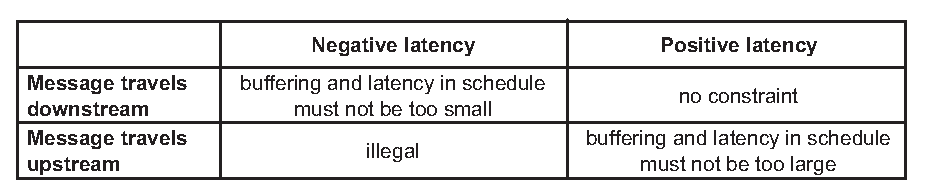
\psfig{file=constraints.eps,width=3.3in}
\vspace{-16pt}
\caption{\small Scheduling constraints imposed by messages.}
%% {\small
%% \begin{tabular}{|r|c|c|} \hline
%% ~ & {\bf Negative latency} & {\bf Positive latency} \\ \hline
%% {\bf Message travels downstream} & buffering and latency in schedule must not be too small & no constraint \\ \hline
%% {\bf Message travels upstream} & illegal & buffering and latency in schedule must not be too big \\ \hline
%% \end{tabular}}
\label{tab:messcons}
\end{center}
\vspace{-18pt}
\end{figure}

An upstream message with negative or zero latency is impossible to
deliver, because the data dependences imply that the target iteration
has already passed when the message was sent.  Conversely, a
downstream message with positive or zero latency imposes no constraint
on the schedule, as the sender has not yet produced the data that is
synchronized with the message.

\paragraph*{Unsatisfiable Constraints}  
Messaging constraints can be unsatisfiable---that is, assuming a
message is sent on every iteration of the sender's work function,
there does not exist a schedule that delivers all of the messages
within the desired latency range.  Such constraints should result in a
compile-time error.  Figure~\ref{fig:infeasible} illustrates two
examples of unsatisfiable constraints.  In
Figure~\ref{fig:infeasible}(a), the latency of the upstream message
from $X$ to $Y$ is is too tight given the actors' I/O rates.  Consider
that $X$ sends a message on its first execution ($n=1$).  The message
should be delivered to $Y$ on iteration $m$, where $m$ is constrained
as follows ($k_1 = k_2 = 1$):
\begin{equation*}
\begin{array}{c}
\sdepf{Y}{X}(n+k_1) \le m \le \sdepf{Y}{X}(n+k_2) \\[1Ex]
\sdepf{Y}{X}(2) \le m \le \sdepf{Y}{X}(2) \\[1Ex]
m = \sdepf{Y}{X}(2)
\end{array}
\vspace{-4pt}
\end{equation*}
The reader can verify that $\sdepf{Y}{X}(n) = \lceil n/3 \rceil$,
which implies that $m=1$.  However, because $X$ is executing its first
iteration, $Y$ must have already fired, so it is too late to deliver
the message.  The smallest legal message latency in this graph is 3,
which will lead to a legal delivery time of $m=2$.  In general, for an
upstream message from $X$ to $Y$ to be satisfiable, its maximum
latency $k_2$ must meet the following condition:
\begin{equation*}
\begin{array}{c}
\forall n \in [1, |{\cal S} \wedge X|]:~~\sdepf{Y}{X}(n) < \sdepf{Y}{X}(n+k_2)
\end{array}
\end{equation*}
That is, for all executions $n$ of actor $X$ in the steady state (see
Section~\ref{sec:calc-sdep}), the current iteration of $Y$
($\sdepf{Y}{X}(n)$) must precede the delivery time
($\sdepf{Y}{X}(n+k_2)$).  This condition is straightforward to check
at compile time once the $\sdep$ information has been computed.  A
similar condition applies to downstream messages.

\begin{figure}[t]
\begin{center}
\psfig{figure=infeasible-messaging2.eps,height=0.66in}
\hspace{0.7in}
\psfig{figure=infeasible-messaging.eps,height=1.43in} \vspace{6pt}

{\tiny ~}{\tiny ~}~{\bf (a)}\hspace{1in}{\bf (b)}~~~{\tiny ~}{\tiny ~}
\vspace{-3pt}
\caption{{\small Examples of unsatisfiable message constraints.  Each
node is annotated with its input and output rate.  Messages are shown
by dotted arrows, drawn from sender to receiver with a given latency.
(a) Constraint is unsatisfiable because latency is smaller than the
communication ratio between $Y$ and $X$, (b) Constraints are
satisfiable in isolation, but unsatisfiable in combination.
\protect\label{fig:infeasible}}}
\end{center}
\vspace{-18pt}
\end{figure}

One can also construct cases where each constraint implied by
messaging is satisfiable, but the set of constraints together is
unsatisfiable.  Figure~\ref{fig:infeasible}(b) shows one such case.
The unsatisfiability is caused by conflicting demands on the buffering
between B and C.  The message from B to C constrains this buffer to
contain at least 10 items, while the message from D to A constrains it
to be empty.  We say that these two constraints {\it overlap} because
the paths from sender to receiver intersect a common actor in the
stream graph.

\paragraph*{Finding a Schedule}
In the presence of overlapping constraints, we leave to future work
the problem of finding a legal execution schedule (if one exists).
Because overlapping constraints can be detected statically, a given
compiler may choose to prohibit overlapping constraints altogether.
%A discussion of the issues involved appears in a
%thesis~\cite{karczma-thesis} by one of the authors.

For the case of non-overlapping constraints, a simple modification to
pull scheduling will always result in a legal schedule (if one
exists).  First, note that a pull schedule always satisfies
constraints imposed by upstream messages; because upstream (receiving)
actors execute as little as possible per execution of the downstream
(sending) actor, a message can be forwarded to the receiver
immediately after sending.  The receiver can then store the message
and process it at the appropriate iteration.  For downstream messages,
the pull scheduler is modified to always execute one iteration of the
upstream (sending) actor before any execution of the downstream
(receiving) actor that would exceed the latency range.  If the
upstream actor needs more inputs to fire, then they can always be
generated by actors that are further upstream (via a recursive call to
the pull scheduling algorithm).

As described in Section~\ref{sec:evaluation}, our compiler uses a
simple implementation of messaging in which each sender or receiver
executes in its own thread and waits for possible messages at
appropriate iterations.  This approach does not depend on producing a
serial ordering of the actors at compile time.

\section{Case Study}
\label{sec:casestudy}

To illustrate the pros and cons of teleport messaging, we implemented
a spread-spectrum frequency hopping radio frontend~\cite{harada02} as
shown in Figure~\ref{fig:fhr-streamit}.  A frequency hopping radio is
one in which the receiver switches between a set of known frequencies
whenever it detects certain tones from the transmitter.  The frequency
hopping is a good match for control messages because the hopping
interval is dynamic (based on data in the stream); it spans a large
section of the stream graph (there is a Fast Fourier Transform (FFT)
with 15 child actors, not shown, between the demodulator and the hop
detector); and it requires precise message delivery.  The delivery
must be precise both to meet real-time requirements (as the
transmitter will leave the current frequency soon), and to ensure that
the message falls at a logical frame boundary; if the frequency change
is out of sync with the FFT, then the FFT will muddle the spectrum of
the old and new frequency bands.

A StreamIt version of the radio frontend with teleport messaging
appears in Figure~\ref{fig:freq1}.  The FreqHoppingRadio pipeline
creates a portal and adds the RFtoIF actor as a receiver (lines 45 and
48 respectively).  The portal is passed to the CheckFreqHop stage,
where four parallel detectors send messages into the portal if they
detect a hop in the frequency they are monitoring (lines 32-35).  The
messages are sent with a latency of 6 to ensure a timely transition.
To make sense of the latency, note that $\sdepf{RFtoIF}{D}(n) = 512*n$
for each of the detector actors $D$.  This comes about because the FFT
stage consumes and produces 512 items\footnote{\small Though the FFT is
256-way, the real and imaginary parts are interleaved on the tape,
leading to an I/O rate of 512.}; each detector fires once per set of
outputs from the FFT, but RFtoIF fires 512 times to fill the FFT
input.  Because of this $\sdep$ relationship, messages sent from the
detectors to RFtoIF are guaranteed to arrive only at iterations that
are a multiple of 512.  This satisfies the design criterion that a
given FFT stage will not operate on data that were demodulated at two
separate frequencies.

Another version of the frequency hopping radio appears in
Figures~\ref{fig:fhr-manual} and~\ref{fig:freq2}.  This version is
functionally equivalent to the first, except that the control messages
are implemented manually by embedding them in the data stream and
introducing a feedback loop.  Because the number of items transfered
around the loop must be constant from one iteration to the next, a
data item is sent whether or not there is a message as part of the
algorithm.  The RFtoIF filter checks the values from the loop on every
iteration; if the value is non-zero, it is treated as a message (the
new frequency), while a value of zero is ignored (no message).  The
I/O rate of the RFtoIF filter has been scaled up to ensure that the
messaging information is received at intervals of 512 iterations (as
in the version with portals).  To achieve the desired messaging
latency of 6 frames, $6*256 = 1536$ items are enqueued on the feedback
path prior to execution.

\begin{figure}[t]
\vspace{-12pt}
\centering
\psfig{figure=fhr-streamit.eps,width=2.841in}
\vspace{-8pt}
\caption{\small Stream graph of frequency hopping radio with teleport messaging.  
A portal delivers point-to-point latency-constrained messages from the
detectors to the RFtoIF stage.
\protect\label{fig:fhr-streamit}}
\vspace{-12pt}
\end{figure}

\begin{figure}[t]
\vspace{-12pt}
\hspace{-0.2in}\psfig{figure=code-freq1.eps,width=3.5in}
\vspace{-24pt}
\caption{\small Frequency hopping radio with teleport messaging.
Arrows depict the path of messages from the sender to the receiver,
via a portal declared in the top-level stream.
\protect\label{fig:freq1}}
\vspace{-12pt}
\end{figure}

%% As described previously, yet another way to approximate the behavior
%% of messaging is with a direct function call from the detector to the
%% RFtoIF stage.  (Though such a call is disallowed in StreamIt, it could
%% be an option in a different programming model.)  While this approach
%% is simple, it does not have any timing guarantees.  Because the sender
%% and receiver are running in parallel, there is no way for the sender
%% to know when in the course of the receiver's execution the message
%% will be received.  This could cause problems both for algorithm
%% development and for the reliability and predictability of software.

\subsection{Discussion}

Teleport messaging offers several benefits compared to a manual
implementation of equivalent functionality.  While embedding messages
in the data stream is equally precise, it involves several tedious
and error-prone changes, not only to the stream graph but also to the
steady-state execution code within the actors.  In particular, the
manual derivation of the loop delay, adjustment of the actor I/O
rates, and implicit interleaving of data items with control messages
has a negative impact on the readability and maintainability of the
code.  Teleport messaging provides the same level of precision, but
with the simplicity of a method call.

Teleport messaging also has advantages from a compiler standpoint.  By
separating the data-intensive code from the control-oriented code, the
common case of steady-state execution is not sacrificed for
the uncommon case of message processing.  There are no ``dummy items''
serving as placeholders in the static-rate channels.  In addition, by
exposing the message latency as part of the language, the compiler can
infer the true dependences between actor firings and reorder the
execution so long as the message constraints are respected.  The
actual message delivery can be implemented in the most efficient way
for a given architecture.

\begin{figure}[t]
\centering
\vspace{-12pt}
\psfig{figure=fhr-feedback.eps,width=3.13in}
\vspace{-10pt}
\caption{\small Stream graph of frequency hopping radio with control
messages implemented manually.  A feedback loop connects the detectors
with the RFtoIF stage, and an item is sent on every invocation to
indicate whether or not a message is present.  The latency and
periodicity of message delivery are governed by the data rates and the
number of items on the feedback
path. \protect\label{fig:fhr-manual}}
\vspace{-12pt}
\end{figure}

A final benefit of teleport messaging is the clean interface provided
by the portals.  Since a portal can have multiple receivers, it is
straightforward to send a message that is delivered synchronously to
two actors in parallel streams.  For example, consider a vocoder (an
encoder for voice signals) that is separately manipulating the
magnitude and phase components of a signal.  If something triggers an
adjustment to the speech transformation (e.g., the speaker
requests a change of pitch) then the mask needs to be updated at the
same time relative to data in both parallel streams.  A portal that
contains both components seamlessly provides this functionality.
Finally, portals are useful as an external programming interface; an
application can export a portal based on an interface type without
exposing the underlying actor implementation.

One aspect of teleport messaging might be considered unusual: the
granularity of message delivery can be affected by changes in
granularity elsewhere in the stream graph.  This is evident in the
frequency hopping radio, as the I/O rate of 512 on the FFT implies
that the RFToIF stage will receive messages from CheckFreqHop at most
once every 512 iterations.  (If the FFT were coarsened to 1024-way,
the granularity of messages in RFToIF would increase accordingly.)  In
this case the behavior is desirable, as messages should not interrupt
frame boundaries.  It seems that in many cases, the I/O rates are
meaningful aspects of the program and their influence on message
granularity is appropriate.  Nonetheless, this non-local influence
might come as a surprise to programmers.  If the FFT granularity is
scaled up for a different reason (e.g., caching behavior), the effects
on message granularity might be unwanted.

This suggests that it might be worthwhile, in future work, to
investigate additional mechanisms for programmers to specify the
messaging contract independently of the declared I/O rates.  For
example, a parent stream could override the I/O rates of a child for
the sake of a given $\sdep$ calculation.  The scheduler would deliver
messages according to the parent's expectation of $\sdep$, or report
an error if such delivery is incompatible with the actual I/O rates.

\subsection{Experimental Evaluation}
\label{sec:evaluation}

We have implemented teleport messaging in the StreamIt compiler
infrastructure~\cite{streamit-asplos}, with a backend that targets a
cluster of workstations.  A StreamIt program is compiled to a set of
parallel threads; if two threads are allocated to different machines,
they communicate via dedicated TCP/IP connections.  Messages are
supported via auxiliary communication channels that transmit two kinds
of signals from senders to receivers: 1) the contents of a control
message, or 2) a {\it credit} that indicates the receiver can execute
some number of iterations before checking for a message again.

Each actor alternates between normal execution and checking for the
exchange of credits.  This serves to throttle the message receiver in
accordance with the constraints (Section~\ref{sec:teleport}), as an
actor will block waiting for credits until the sender has reached a
given point in its execution.  The compiler calculates the $\sdep$
information and schedules the exchange of credits to make sure that
the timing constraints are respected.  When a message is sent, it is
tagged with the iteration number during which the receiver should
process it; this is also calculated using $\sdep$ in the compiler.

%% In our implementation, each actor maintains an iteration number which
%% serves to synchronize message delivery. A message from a sender $A$ to
%% a receiver $B$ is tagged with the iteration number in $B$ when the
%% message must be processed. The iteration number is calculated by the
%% sender using the $\sdep$ relation and the specified message latency.

%% The compiler automatically schedules the exchange of credits between
%% actors when it derives an execution of the stream graph. Our
%% communication layer guarantees that messages are received before
%% credits and hence processed during the appropriate execution step.
%% For messages sent downstream with zero or positive latencies, we do
%% not use the credit system, and assume that the messages arrive as fast
%% or faster than the data items exchanged between the two actors. This
%% assumption is safe since, due to the data dependences, a downstream
%% filter cannot get ahead of an upstream actor.

%Our compiler maps threads to workstations using a dynamic programming
%algorithm.  The algorithm aims to reduce the overall application
%bottleneck, thereby maximizing the steady-state throughput of the
%output actor (i.e., most downstream actor in the stream graph).
%In our experiments, we are interested in quantifying two performance
%metrics: throughput and communication overhead.  For the purpose of
%this paper, throughput is defined as the number of outputs produced
%per unit of time, and communication overhead reflects the quantity of
%data transmitted between workstations.
%The StreamIt compiler automatically partitions an input program into a
%set of threads that are mapped to the workstations and then run
%concurrently.

We chose a cluster-based evaluation for two reasons.  First, many
streaming applications run on the server side (e.g., cell phone base
stations, radar processing, HDTV editing) and require large
computational resources. Second, clusters provide a simple abstraction
for distributed and parallel computing---multiple program counters,
and distributed memories---which is at the heart of emerging
multi-core architectures for embedded, desktop, and server computing.

The teleport implementation of the frequency hopping radio was
compiled into 29 threads whereas the alternate version using a
feedback loop results in 33 threads.  Each thread corresponds to a
single actor (there are more threads than appear in
Figures~\ref{fig:fhr-streamit} and~\ref{fig:fhr-manual} because the
FFT stage is a pipeline composed of several actors).  The thread
mapping is done using a dynamic programming algorithm that aims to
reduce the overall bottleneck, thereby maximizing throughput (outputs
per unit time).  Threads are assigned to one of sixteen 750Mhz
Pentium~III workstations, each with a 256Kb cache.  The machines are
interconnected using a fully switched 100Mb network.

%
\begin{figure}[t]
\vspace{-12pt}
\hspace{-0.2in}\psfig{figure=code-freq2.eps,width=3.5in}
\vspace{-20pt}
\caption{\small Frequency hopping radio with manual feedback loop for
event handling.  Lines that differ from Figure~\ref{fig:freq1} are
marked with an asterisk. \protect\label{fig:freq2}}
\vspace{-12pt}
\end{figure}

\clearpage
\noindent
%

Figure~\ref{fig:fhr-throughput} shows the measured throughput
($y$-axis) for various cluster sizes.  Note that due to the limited
parallelism in the two implementations of the frequency hopper,
cluster configurations with more than five workstations lead to
negligible performance gains. From the data, we can observe that
teleport messaging achieves a maximal throughput that is 49\% better
than its counterpart.  We attribute this speedup primarily to reduced
communication overhead.  A detailed analysis of the results indicates
that teleport messaging reduces the number of items communicated by
35\%.  While the feedback loop version sends a message placeholder on
every iteration, teleport messaging uses credits to allow the receiver
to execute several iterations at a time without checking for messages.
The amount of communications savings is dictated by the message
latency, as larger latencies allow for a less frequent exchange of
credits.

\begin{figure}[t]
\vspace{-10pt}
\psfig{figure=throughput-graph.eps,width=3.3in}
\vspace{-20pt}
\caption{\small Throughput as a function of the number of workstations
in the cluster. 
\protect\label{fig:fhr-throughput}}
\vspace{-6pt}
\end{figure}

%% There are two factors contributing to this speedup.  First, teleport
%% messaging exposes more parallelism in the application, as the compiler
%% understands that the RFtoIF stage can execute ahead of each
%% CheckFreqHop stage, so long as the message latency is respected.
%% In contrast, the manual implementation sends an item along the
%% feedback path on every iteration, thereby restricting RFtoIF to only
%% process one frame at a time.  This explains why the speedup improves
%% as the number of processors increases: the extra parallelism is being
%% utilized.  A second factor that could contribute to the improved
%% performance is the reduced communication overhead.  

% implementation goes here -- cluster and constrained
\section{Related Work}
\label{sec:related-work}

The work most closely related to ours comes from the fields of
heterogeneous modeling, program slicing, and domain-specific
languages.

The models of computation in our system are closely related to those
explored in the Ptolemy project for heterogeneous
design~\cite{ptolemy03overview}.  As part of this effort, Lee et
al. have established the Synchronous Dataflow (SDF)
paradigm~\cite{LM87-i} and have developed hybrid models that
incorporate Dynamic Dataflow (DDF, in which the I/O rates of actors
are fully dynamic).  Boolean Dataflow (BDF)~\cite{ha97profile} is a
compromise between these two extremes; it computes a parameterized
schedule of the graph at compile time, and substitutes runtime
conditions to decide which paths are taken.  The performance is nearly
that of SDF while keeping some flexibility of DDF.  

Teleport messaging shares the motivation of BDF, but is different in
its approach.  We believe that control messages represent a distinct
and well-behaved class of dynamic communication in which a parameter
is ``pushed'' into the receiving actor in an asynchronous way.
Because the message handlers do not access the I/O channels of the
receiving actor, their irregular invocations do not interfere with a
given static schedule.  Instead, the schedule is constrained only by
the latency of control messages; if a message does not show up in the
allotted window, then the receiving actor can go ahead with its
high-bandwidth schedule.  This is the distinction in the computational
model.  In addition, the static/dynamic integration offered by our
system is integrated with language features that support the model.

Program slicing identifies the set of statements in a program that a
given statement might depend on.  There is a rich history of work in
program slicing; see Tip~\cite{tip95slice} for a comprehensive review.
Many program slicing techniques rely on the Program Dependence Graph
as described by Horwitz et al.~\cite{hrb88pdg}.  Program slicing has
been applied for debugging, testing, and program analysis.  In many
respects, $\sdep$ analysis can be thought of as a slicing technique
for Synchronous Dataflow graphs.  Because the input domain is
restricted (in particular, because of the absence of control flow and
recursion), the $\sdep$ calculation can make stronger guarantees than
slicing analyses for general procedural languages; $\sdep$ is
decidable, exact, and admits a compact representation in terms of the
steady state schedule.

Pugh and Rosser present an iteration-based slicing
algorithm~\cite{pugh97slice} to identify the dynamic instances of
statements (in terms of their loop iteration) that effect a given
value.  This bears some similarity to stream dependence analysis, as
$\sdepf{A}{B}(n)$ represents the last iteration of actor $A$ that
affected the $n$th iteration of actor $B$.
However,~\cite{pugh97slice} focuses on the problem of computing the
transitive closure of dependences in loops, in which some iterations
do not depend on others.  We are not interested in this question, as
we assume that all actor invocations depend on their previous
invocations; $\sdep$ addresses the question of finding only the most
recent invocation that is relevant.  Moreover, our motivation differs
from the slicing community, as we apply $\sdep$ to enrich the
semantics of language features.  To the best of our knowledge, slicing
has not been applied in this way before.

There are many domain-specific stream languages in addition to
StreamIt.  Streams have a long history in the programming languages
community, with influences from dataflow, CSP, synchronous and
functional languages; see Stephens~\cite{survey97} for a review.
Languages of recent interest include Brook~\cite{brook04},
Cg~\cite{cg03}, StreamC/KernelC~\cite{imagine03ieee},
Spidle~\cite{spidle02}, Occam~\cite{occammanual}, Sisal~\cite{sisal},
and Parallel Haskell~\cite{ph}.  The principle differences between
StreamIt and these languages are $(i)$ StreamIt adopts the SDF model of
computation, which narrows the application class but enables powerful
optimizations, $(ii)$ StreamIt's support for a ``peek'' construct that
inspects an item without consuming it from the channel, $(iii)$ the
single-input, single-output hierarchical structure that StreamIt
imposes on the stream graph, and $(iv)$ teleport messaging as
described in this paper.

\section{Conclusions and Future Work}
\label{sec:conclusion}

This paper makes two contributions.  First, it introduces teleport
messaging: a powerful language construct enabling precise message
delivery between nodes of a distributed stream program.  In comparison
with other methods to implement messaging functionality in a
Synchronous Dataflow model, teleport messaging is arguably more
readable, more robust, and easier to maintain.  In addition, our
implementation of teleport messaging in the StreamIt compiler results
in a 49\% performance improvement for a frequency hopping radio
running on a cluster of workstations.  Like several other declarative
language constructs, teleport messaging improves performance by
exposing the true dependences to the compiler and allowing it to
optimize the communication.

%% We outlined several possible applications of $\sdep$, including
%% latency constraints, debugging, speculation, and program analysis, and
%% we look forward to pursuing these directions in the future.

Second, this paper formulates $\sdep$, a natural and useful dependence
representation for the streaming domain.  While this paper applies
$\sdep$ to a new language construct, we envision other applications as
well.  For example, $\sdep$ could be used in a debugger to identify
which iterations of one actor are affecting a given iteration of
another.  In a software-based speculation system~\cite{frank-thesis},
$\sdep$ could be applied to trace the effects of a failed prediction
and to roll back the appropriate actor executions.  Analogous to
representations such as dependence levels~~\cite{AK82}, direction
vectors~\cite{wolfe82}, and dependence polyhedra~\cite{Irig88} for
scientific programs, $\sdep$ provides dependence information that
could be used to test or verify program transformations.  Also,
$\sdep$ offers a new method for measuring latency in a stream graph.

There are some limitations in the current study that are fertile
grounds for future research.  First, our formulation of $\sdep$
requires a directed path in the stream graph between the actors in
question.  We are generalizing $\sdep$ to actors that run in parallel
by leveraging their data dependences with common predecessors
(upstream) or successors (downstream).  Second, as detailed in
Section~\ref{sec:constraints}, we do not solve the general scheduling
problem that incorporates overlapping constraints from teleport
messaging; even determining whether or not a set of constraints is
feasible (especially during the initialization
schedule~\cite{karczma-thesis}) seems to be an interesting question.
Third, in the current model only actors can send and receive messages.
We are extending this into a hierarchical model where stream
containers (such as pipelines) can also receive events and dispatch
them precisely to other streams.  Finally, our approach relies on the
static communication rates present in SDF.  It is interesting to
consider teleport messaging in a more dynamic context; for example,
downstream non-negative latency messages could be supported by
embedding messages in data items, while other messages might require
speculative delivery or modified timing contracts.

Our work can be viewed as integrating dynamic behavior into a static
dataflow language.  Our insight is that there is a class of control
messages that only adjust parameters in the target actor; they do not
otherwise affect the input or output channels upon delivery.  This
model enables a hybrid scheduling scheme in which the steady-state
dataflow is exactly orchestrated at compile time, but there are
windows in which a message could adjust an internal field of an actor
between its execution steps.  We consider this to be a promising
avenue for creating a unified development environment that captures
all aspects of stream application development without sacrificing
either performance or programmability.

\section{Acknowledgments}

We are very grateful to Jasper Lin for insightful comments on this
paper.  We also thank David Maze, Jasper Lin, and Michael Gordon for
assistance with the StreamIt implementation, and the anonymous
reviewers for their helpful comments.  The StreamIt project is
supported by DARPA grants PCA-F29601-03-2-0065 and
HPCA/PERCS-W0133890; NSF awards CNS-0305453 and EIA-0071841; and the
MIT Oxygen Alliance.


{\small
%  \bibliographystyle{abbrv}
%  \bibliography{references}
\begin{thebibliography}{10}

\bibitem{ph}
S.~Aidtya, Arvind, L.~Augustsson, J.-W. Maessen, and R.~S. Nikhil.
\newblock {Semantics of pH: A parallel dialect of Haskell}.
\newblock In {\em Haskell Workshop}, 1995.

\bibitem{AK82}
J.~Allen and K.~Kennedy.
\newblock {PFC: A program to convert Fortran to parallel form}.
\newblock {\em Proc. of the IBM Conf. on Parallel Computing and Scientific
  Computations}, 1982.

\bibitem{BELP96}
G.~Bilsen, M.~Engels, R.~Lauwereins, and J.~Peperstraete.
\newblock Cyclo-static dataflow.
\newblock {\em IEEE Trans. on Signal Proc.}, 1996.

\bibitem{brook04}
I.~Buck, T.~Foley, D.~Horn, J.~Sugerman, K.~Fatahalian, M.~Houston, and
  P.~Hanrahan.
\newblock {Brook for GPUs: Stream Computing on Graphics Hardware}.
\newblock In {\em SIGGRAPH}, 2004.

\bibitem{spidle02}
C.~Consel, H.~Hamdi, L.~Reveillere, L.~Singaravelu, H.~Yu, and C.~Pu.
\newblock {Spidle: A DSL Approach to Specifying Streaming Applications}.
\newblock Technical report, LABRI Research Report 1282-02, 2002.

\bibitem{conte97}
T.~M. Conte, P.~K. Dubey, M.~D. Jennings, R.~B. Lee, A.~Peleg, S.~Rathnam,
  M.~Schlansker, P.~Song, and A.~Wolfe.
\newblock Challenges to combining general-purpose and multimedia processors.
\newblock {\em IEEE Computer}, 30(12), 1997.

\bibitem{dief97}
K.~Diefendorff and P.~K. Dubey.
\newblock How multimedia workloads will change processor design.
\newblock {\em IEEE Computer}, 30(9), 1997.

\bibitem{frank-thesis}
M.~Frank.
\newblock {\em SUDS: Automatic Parallelization for Raw Processors}.
\newblock PhD thesis, MIT, 2003.

\bibitem{sisal}
J.~Gaudiot, W.~Bohm, T.~DeBoni, J.~Feo, and P.~Mille.
\newblock {The Sisal Model of Functional Programming and its Implementation}.
\newblock In {\em Proc. of the 2nd Aizu Int. Symp. on Parallel
  Algorithms/Architecture Synthesis}, 1997.

\bibitem{streamit-asplos}
M.~Gordon, W.~Thies, M.~Karczmarek, J.~Lin, A.~S. Meli, A.~A. Lamb, C.~Leger,
  J.~Wong, H.~Hoffmann, D.~Maze, and S.~Amarasinghe.
\newblock {A Stream Compiler for Communication-Exposed Architectures}.
\newblock ASPLOS, 2002.

\bibitem{ha97profile}
S.~Ha and E.~A. Lee.
\newblock Compile-time scheduling of dynamic constructs in dataflow program
  graphs.
\newblock {\em IEEE Trans. on Computers}, 6, 1997.

\bibitem{harada02}
H.~Harada and R.~Prasad.
\newblock {\em Simulation and Software Radio for Mobile Communications}.
\newblock Artech House, 2002.

\bibitem{hrb88pdg}
S.~Horwitz, T.~Reps, and D.~Binkley.
\newblock Interprocedural slicing using dependence graphs.
\newblock 1988.

\bibitem{occammanual}
{Inmos Corporation}.
\newblock {\em {Occam 2 Reference Manual}}.
\newblock Prentice Hall, 1988.

\bibitem{Irig88}
F.~Irigoin and R.~Triolet.
\newblock {Supernode partitioning}.
\newblock In {\em {POPL}}, {1988}.

\bibitem{imagine03ieee}
U.~J. Kapasi, S.~Rixner, W.~J. Dally, B.~Khailany, J.~H. Ahn, P.~Mattson, and
  J.~D. Owens.
\newblock Programmable stream processors.
\newblock {\em IEEE Computer}, 2003.

\bibitem{karczma-thesis}
M.~A. Karczmarek.
\newblock {Constrained and phased scheduling of synchronous data flow graphs
  for StreamIt language}.
\newblock Master's thesis, MIT, 2002.

\bibitem{kirkpatrick97}
S.~Kirkpatrick.
\newblock Multimedia's impact on computer architecture.
\newblock Presentation, Harvard University Colloquium Series, May 1997.

\bibitem{ptolemy03overview}
E.~A. Lee.
\newblock {Overview of the Ptolemy Project}.
\newblock Technical report, Tech Memo UCB/ERL M03/25, UC Berkeley, 2003.

\bibitem{LM87-i}
E.~A. Lee and D.~G. Messerschmitt.
\newblock Static scheduling of synchronous data flow programs for digital
  signal processing.
\newblock {\em IEEE Trans. on Computers}, January 1987.

\bibitem{cg03}
W.~R. Mark, R.~S. Glanville, K.~Akeley, and M.~J. Kilgard.
\newblock {Cg: A System for Programming Graphics Hardware in a C-like
  Language}.
\newblock In {\em SIGGRAPH}, 2003.

\bibitem{pugh97slice}
W.~Pugh and E.~Rosser.
\newblock Iteration based slicing and its application to communication
  optimization.
\newblock In {\em Proc. of the Int. Conf. on Supercomputing}, 1997.

\bibitem{Rix98}
S.~Rixner, W.~J. Dally, U.~J. Kapani, B.~Khailany, A.~Lopez-Lagunas, P.~R.
  Mattson, and J.~D. Owens.
\newblock {A Bandwidth-Efficient Architecture for Media Processing}.
\newblock In {\em HPCA}, Dallas, TX, November 1998.

\bibitem{survey97}
R.~Stephens.
\newblock {A Survey of Stream Processing}.
\newblock {\em Acta Informatica}, 34(7), 1997.

\bibitem{streamitcc}
W.~Thies, M.~Karczmarek, and S.~Amarasinghe.
\newblock {StreamIt: A Language for Streaming Applications}.
\newblock In {\em {Proc. of the Int. Conf. on Compiler Construction (CC)}},
  {2002}.

\bibitem{tip95slice}
F.~Tip.
\newblock A survey of program slicing techniques.
\newblock {\em Journal of Programming Languages}, 3(3), 1995.

\bibitem{wolfe82}
M.~Wolfe.
\newblock {\em Optimizing Supercompilers for Supercomputers}.
\newblock PhD thesis, University of Illinois, Urbana-Champaign, 1982.

\end{thebibliography}

}
\end{document}
